\section{Skylines: Demystifying Network Resource Islands with Virtual Landmarks}

``What's in a name?" --- in the context of networking, quite a lot! IP addresses and prefixes
indicate to routers where particular interfaces or subnets reside in the greater Internet
\cite{bgp}. Domain
names offer a simple, human-readable overlay for the complicated, often multiplexed addressing
scheme underneath \cite{dns}. Autonomous system (AS) numbers often help to distingish one network
from another \cite{asn}.
Names and labels such as these, whatever form they take, allow us to organize immense network spaces
with manageable and descriptive abstractions.

Unfortunately, a single name is often not enough. One machine can be described in terms of all of
the examples listed above, and more. This is because it is important that names carry information
relavant to the specific way in which they will be used. Routers are unable to direct traffic with
domain names, just as humans cannot be expected to remember the plethora IP addresses they access
every day. While it is intuitive that no labeling system is applicable across all possible
dimensions, in practice, this fact is often taken for granted or neglected entirely.

In this project, I challenge the careless application of conventional client labeling schemes in
Internet measurement experiments, particulary those subject to the effects of DNS redirection and
CDN PoP (point of presence) catchment formation. I uncover and quantify the degree of misalignment
between experimentally determined aggregate catchments and labels often assumed to indicate
``similarity" between clients --- country, AS number, announced BGP prefix, and /24 subnet --- and
use this to design the Skyline model, a grouping system which describes clients' relative distances
from each other in terms of their \emph{common network resource exposure} (CNRE). Describing clients in such
terms highlights what should be a chief concern in large scale Internet measurement platforms and
network optimization efforts: the sets of clients actually being directed the same resources.

In order to develop the Skyline model, I performed an exhaustive set of measurements to frame
client experience on a per \emph{site} basis. In my completed, preliminary work, I capture a
snapshot of both DNS resolutions and latency measurements toward the 304 domains that appeared most
frequently in the top 2441 most popular webpages. My measurements span over 10,000 unique
clients spread across 185 countries and 3637 autonomous systems. I performed over 52 million pairwise
comparisons with the results of these measurements to arrive at the foundation of what I have
coined the ``Skyline model". 

With this project, I make the following contributions, including those I expect to stem from
proposed work, which I have designated with (\emph{p})

\begin{itemize}\parskip0pt \parsep0pt
    \item I perform a large exploration of client network performance on a per webpage level. My
        raw results are publically available on the RIPE Atlas platform.
    \item (\emph{p}) I quantify the degree of misalignment between conventional grouping schemes
        and aggregate catchments.
    \item (\emph{p}) I introduce the Skyline model, a client grouping scheme that reflects the
        extent of CNRE.
    \item (\emph{p}) Using the Skyline model, I identify and analyze network resource islands --- 
        sets of clients with very high degrees CNRE. 
\end{itemize}

% RELATED WORK and PROBLEM FRAMING
\subsection{Problem Space and Related Work} \label{skyspace}

This projects aims to gain an understanding of which clients are directed to the same set of
resources across many distinct domains. Its most direct and immediate use case is influencing probe
selection in large scale Internet measurements. For researchers, likely unaware of the relatively
hidden allocation schemes of the wide array of CDN platforms and other large content distributors,
it is difficult to determine, a priori, the degree of similarity between clients. Knowledge of
whether there is a high probability that a pair of clients are being directed to altogether
different resources may be significant to their experiment design. This approach to experiment
design is in line with RIPE Atlas, one of the largest client based measurement platforms,
which maintains
an exhaustive set of tags on all of their clients in order to help researchers and network operators
filter and refine the set selected for their experiment \cite{ripe-atlas}. Further, more abstract
applications may include, but are not limited to, distributed denial of service mitigation
\cite{anycastvsddos} and CDN node deployment \cite{35590, Tariq}.

The most similar body of related work involves anycast CDN catchment analysis, which aims to
investigate the set of clients routed towards particular CDN points of presence (PoPs)
\cite{Calder2015, anycastvsddos, vdmscatchment}. My work differs significantly in scope: to my
knowledge, I am the first investigate what I refer to as \emph{aggregate catchments}, the joint
behavior of many anycast CDN catchments and unicast CDN targets, spread across many content
distribution platforms. Conversely, this related body work either focuses on individual platforms or
specific services \cite{Calder2015, anycastvsddos, vdmscatchment}. 

Several authors have attempted to discover the topology of large CDN platforms through large scale
measurement studies \cite{webcart, Calder2013, benson11}. While their findings are potentially of
use in this project, their goals and contributions run parallel to what I aim to accomplish. They
seek to identify the properties and locations of CDN resources; conversely, I seek to identify the
target pools (sets of clients) of overlapping CDN resource catchments \cite{webcart, Calder2013,
benson11}. Other work close to this space investigates the performance of a particular CDN
deployment scheme \cite{ecs15sigcomm}. 


% APPROACH

\subsection{Experiment Overview} \label{oversky}

I aim to establish a baseline by which to compare client labeling systems relative to how well they
capture the similarity of clients with regards to their DNS query answers across a large set of
domains. Clients exposed to the same set of resources should appear to be similar and thus grouped
together by a labeling scheme. Likewise, clients exposed to different resources should appear
disimilar. With this in mind, I opt to use the Jaccard index as inspiration for a simple distance
measure, which I will refer to as closeness. Closeness is explicitly defined in Section
\ref{closeness}.
Essentially, clients with high closeness scores have a large number of network resources in common
(a high degree of CNRE). 

In Section \ref{skyfinds}, I calculate pairwise closeness scores for thousands of clients spread across the
globe. I then group results by a series of conventional naming systems (prefix, /24, AS number, and
country) for further analysis. The continuity of possible closeness values --- which span from 0 to
1 --- give us a mechanism by which we can gauge how well the various labeling schemes are aligned
with the degree overlap in clients' resource exposure. If a labeling scheme is well aligned, we
should be able to expect clients with the same label to be directed to most of the same
endpoints. 

Given that closeness is a distance measure, it may be possible to derive some manner of grouping
from the matrix of pairwise results. In Section \ref{propsky}, I propose applying clustering techniques to
the dataset to gain an understanding of the broader relationship between clients in terms of their
closness. This manner grouping clients will form the basis of what I refer to as the Skyline model.

\subsubsection{Closeness Definition} \label{closeness}

Consider two clients, $p$ and $q$,  who have each resolved $d$ domains, taking the first answer from
each query.  Suppose I were to compare the each client's remaining answer for the first domain,
$d_0$. If the clients were directed to the same resource, client $p$'s answer, $A_0p$, should match
client $q$'s answer, $A_0q$. If I were to continue performing such comparisons across all $d$
domains, I would arrive with a list of booleans, attributing matches result in true values and
mismatches to false.  I define the closeness of two clients as $t / d$, where $t$ is the number of
true values from the list of booleans. 

For now and through my preliminary experiements, I consider only answers within the
same /24 prefix to be \emph{matching}, as /24 is generally the largest routable prefix in IPv4.
However, it is worth noting that it is very possible for large datacenters to include multiple /24
blocks or smaller prefixes. I address this further in the Proposal portion of this document.

% DATA OVERVIEW
\subsection{Measurement Data Collection} \label{sky:data}

Any attempt to investigate grouping requires a dataset with a
uniquely broad scope: not only breadth --- a diverse set of clients --- but also depth --- many
clients from each, yet to be uncovered, group. In addition, we are required to minimize the
temporal spread of the measurements, as network resource allocation is known to change over time.
And finally, to ensure that my experiments cover to the most relevant space possible, it is
important that I particularly target popular domains, which are the target of the vast majority
of DNS resolutions and Internet traffic.

\subsubsection{Domain Collection}

I first obtained the top 10,000 most frequently resolved domains from Cisco's Umbrella Top
1-Million list. While this list captures popularity, it does not reflect what a client might
experience browsing a given site; the relationships between domains are not provided. In order to
obtain a more comprehensive dataset, I needed to extract webpage level statistics. I attempted to
crawl the landing page of these domains, and of the 10,000, 2,441 domains pointed to loadable
websites. I generated a HAR file (HTTP Archive) for each page, using a fully functional
installation of Google Chrome with JavaScript enabled. Note that I allowed each page to load for
several seconds, esuring that any AJAX loaded objects were captured by the HAR file. From the
collected HAR files, I determined the domains from which each loaded web object was downloaded and
calculated the frequency with which each web object domain appeared across all visited pages. 

\subsubsection{Measurements}

In order to meet the necessary client space coverage, I deployed the
experiment over the RIPE Atlas platform. I launched measurements from 10,274 distinct clients, hailing
from 185 countries and 3637 autonomous systems. Throughout the month of June, 2018, I deployed ping
measurements from each probe to each of the object domains obtained in the previous subsection, with
each ping preceded by a local DNS resolution performed by the client. I obtained results for the
top 304 most commonly occuring object domains. 

I note here that, due to the scale my experiments, it was important to respect measuremnent
deployment rate limits in an effort to avoid inadvertant denial of service attacks. As a result,
performing a measurement across all probes for a single domain consumed several hours, and,
therefore, results from a pair of clients to that domain may be separated by a similar amount of
time. Based on findings from CITE et al, where domain to IP mapping was shown to change slowly over
time, I believe these effects of these time gaps to be sufficiently negligible for this project. 

\subsubsection{Raw Dataset Features}

\begin{figure*}
    \center
            \begin{subfigure}[b]{.7\linewidth}
                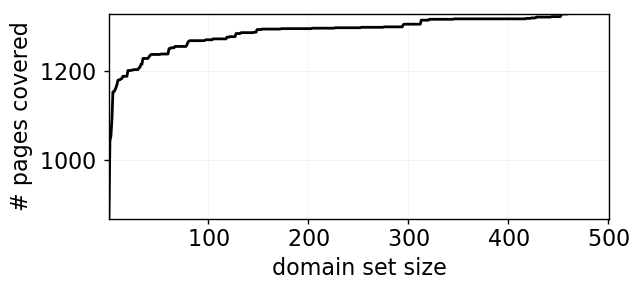
\epsfig{file=figs/num_sites_covered_by_top_n_doms.png, width=1\linewidth}
                \caption{Number of pages that include at least one of the domains from a domain set
                of size $x$.}
                \label{num_pages}
            \end{subfigure}
            \begin{subfigure}[b]{0.7\linewidth}
                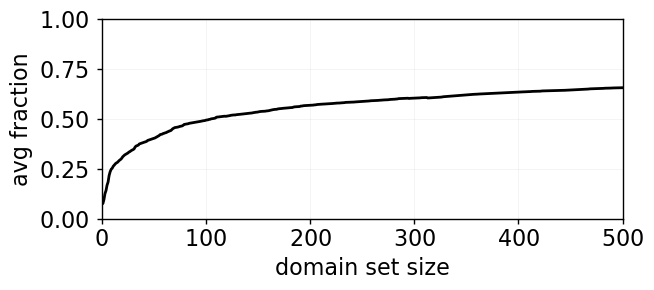
\epsfig{file=figs/fraction_links_covered_by_top_n_doms.png, width=1\linewidth}
                \caption{Mean fraction of links covered on pages that include at least one of the
                domains from a domain set of size $x$}
                \label{frac_links}
            \end{subfigure}
\end{figure*}

Before moving forward, I take a brief moment to explore the properties of my raw dataset in order
to provide the reader appropriate context. First, I illustrate the relative importance of each
domain in the dataset. In Figure \ref{num_pages}, I plot how the number of webpages with at least
one of the
considered domains the number of considered domains increases. As seen in the plot, the first
NUM most popular domains span well over a thousand webpages. Meanwhile, the marginal beneifit of
each additional domain considered rapidly decreases. Part of this is due to overlap; the set of
sites covered by domain $N$ may have significant overlap with the set of pages covered by domains 1
through $N-1$. This is clear from Figure \ref{frac_links}, which plots the average fraction of links from each
webpage (within the pages covered by domains 1 through $N$). After NUM domains have been considered,
over 50\% of links on the pages covered are in the set of considered domains. Based on this, I
consider the 304 domains measured in the experiment to be a fairly representative of approximation
of client browsing experience on a per site basis. 

In addition to this, it is worth noting that for many clients, measurements were only obtained for
a subset of the 304 domains. This results primarily from churn in the set of clients available on
the platform over course of experiment. Other possible explanations may include oneoff DNS
resolution errors or other localized issues such as censorship. Therefore, I update the closeness
calculation so that $d$ represents the size of the set of domains measured by \emph{both} clients
being compared. If $d$ is 0, no comparison is made. For most comparisons, $d$ is high (upwards of
200). I discuss this further in Section \ref{propsky}.

% PRELIMINARY FINDINGS
\subsection{Early Findings} \label{skyfinds}

In this section, I present the results of my preliminary analysis. Before proceeding, we take a
moment to describe how closeness was obtained between \emph{labels}. This is most easily expressed
with the following illustrative example, where labels of interest are drawn from the
``country"-based labeling scheme (I trust that the reader can easily apply this method to AS
number, prefix, and /24): Consider two sets of clients from two countries, $P$ and $Q$. I perform
pairwise comparisons for all combinations containing exactly one client from each country.  From
this, I define the closeness of $P$ and $Q$ as the median of their set of client-pair closeness
scores. I use the median in an effort to avoid potentially noisy outlier behavior. Note, I allow
for $P$ and $Q$ to be the same label, as I am also interested in the closeness of clients in the
same group. All comparisons in this section use the described group aggregates for comparison. 

\begin{figure*}
    \center
            \begin{subfigure}[b]{.7\linewidth}
                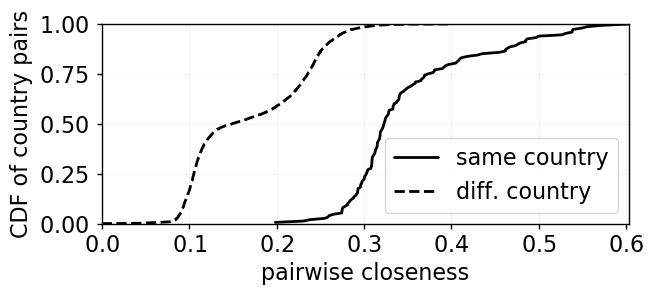
\epsfig{file=figs/country_cdf.png, width=1\linewidth}
                \caption{country}
            \end{subfigure}
            \begin{subfigure}[b]{.7\linewidth}
                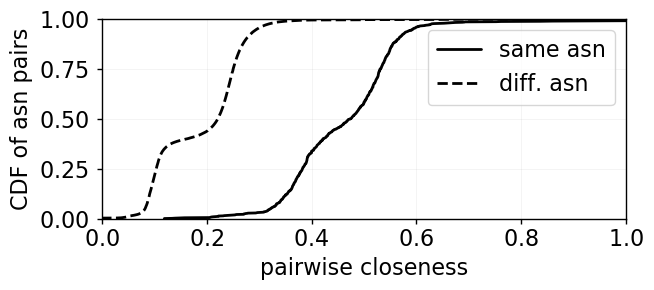
\epsfig{file=figs/asn_cdf.png, width=1\linewidth}
                \caption{asn}
            \end{subfigure}
            \begin{subfigure}[b]{.7\linewidth}
                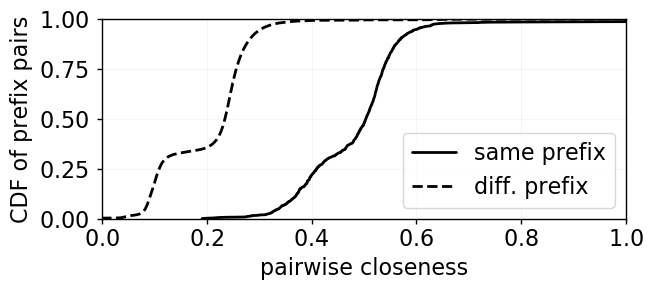
\epsfig{file=figs/prefix_cdf.png, width=1\linewidth}
                \caption{BGP prefix}
            \end{subfigure}
            \begin{subfigure}[b]{.7\linewidth}
                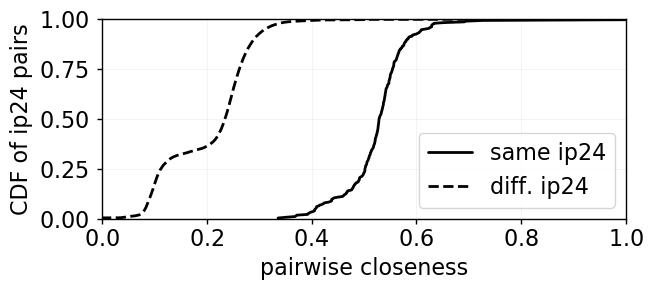
\epsfig{file=figs/ip24_cdf.png, width=1\linewidth}
                \caption{/24 subnet}
            \end{subfigure}
            \caption{CDFs of aggregate group closeness.}
            \label{closecdf}
\end{figure*}

Figure \ref{closecdf}, plots pairs of CDFs that contrast the closeness of clients in the same group with
that of different groups. Across all examined labeling schemes, clients in the same group tend to be
closer than those of different groups. However, the CDF pairs overlap to some extent, indicating
that there is generally no magic threshold at which we can assume clients to be in the same group.
More importantly, each curve spans over 30\% of possible closeness values, rendering it difficult
infer closeness based on matching or mismatching labels. It is possible that this is partially due
to the non-binary nature of the factors that determine closeness. Specifically, there likely a
gradient where closeness gradually increases or decreases as you move along some dimension in
client space. 

I draw attention to the fact that most of the observed closeness scores, even for clients in the
same /24, fell well below 1. This may partially stem from the fact that I define only DNS answers
with the \emph{same} /24 as a ``match" in closeness calculation. Such an approach makes each
comparison susceptible to the effects of load balancing and other dynamic labeling schemes. This
reflects the findings of previous work showing that even queries performed by the exact
same client may span a large range of possible answers, particularly for popular domains, CITE. 
\begin{figure*}
    \center
        \mbox{
            \begin{subfigure}[b]{.5\linewidth}
                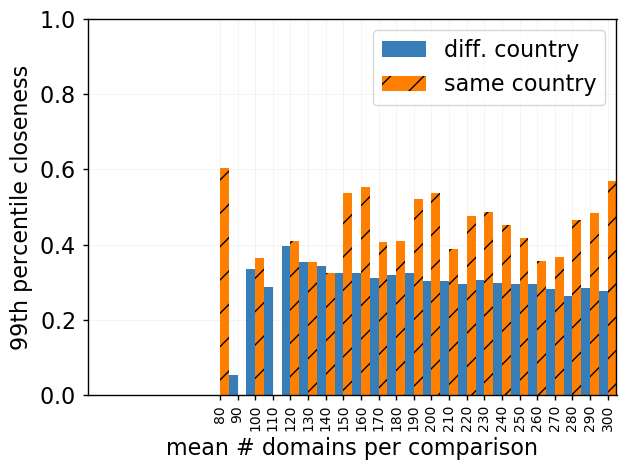
\epsfig{file=figs/country_percentile_vs_counts.png, width=1\linewidth}
                \caption{country}
            \end{subfigure}
            \begin{subfigure}[b]{.5\linewidth}
                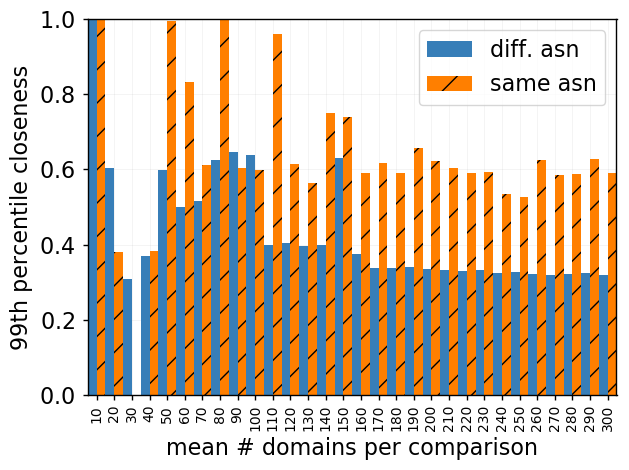
\epsfig{file=figs/asn_percentile_vs_counts.png, width=1\linewidth}
                \caption{asn}
            \end{subfigure}
        }
        \mbox{
            \begin{subfigure}[b]{.5\linewidth}
                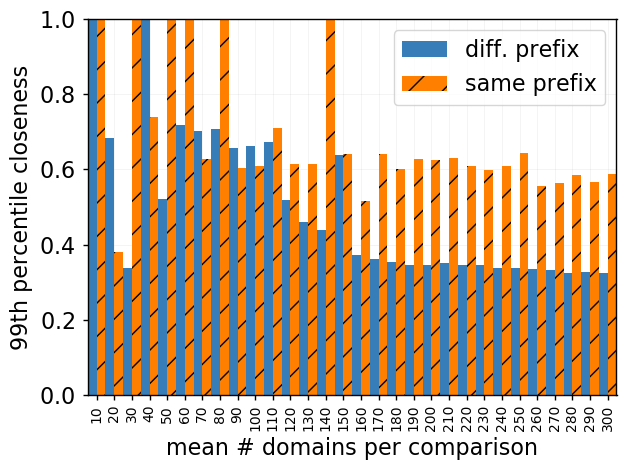
\epsfig{file=figs/prefix_percentile_vs_counts.png, width=1\linewidth}
                \caption{BGP prefix}
            \end{subfigure}
            \begin{subfigure}[b]{.5\linewidth}
                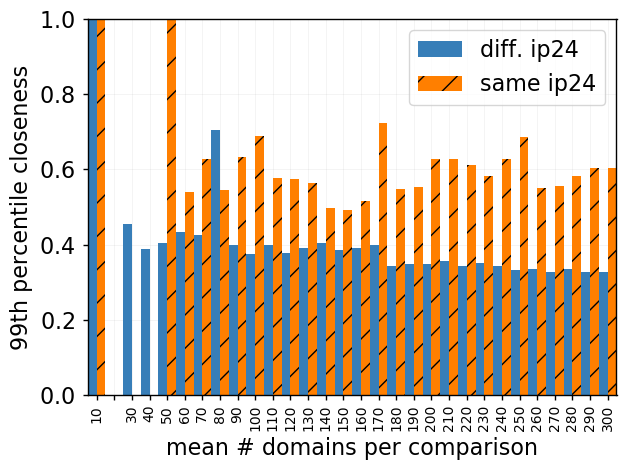
\epsfig{file=figs/ip24_percentile_vs_counts.png, width=1\linewidth}
                \caption{/24 subnet}
            \end{subfigure}
        }
            \caption{Bar plots of aggregate group closeness vs number of average number of domains
            used in closeness calculation for group pair.}
            \label{closecount}
\end{figure*}

As explained in Section \ref{closeness}, the size of $d$, the set of domains compared, varies across client
pairs. Figure \ref{closecount} shows how closeness scores for label pairs change with respect to the
average $d$ of their respective client pairs. Each bar correspends to a bin where $d$ ranges from
$x-10$ to $x$, and the height of the bar is the 99th percentile of all group aggregate pair scores
in that bin. Unlabeled tickmarks and bars with height 0 indicate empty bins (not zero values). I make the following
two observations. First, I see that as the number of domains compared increases, the closeness of
distinct labels \emph{decreases}; in other words, it becomes more apparent that clients are in
different groups as more domains are introduced to the closeness calculation. It is worth noting
however, that there seems to be a decrease in the marginal effect of each additional domain. Second,
I observe that closeness of clients with the same label \emph{stabilizes} after some number of
domains have been compared; it ceases to follow any general upward or downward trend.

Interestingly, in Figure \ref{closecount} it becomes acutely apparent that closeness does not
tend to increase with finer group granularity when using conventional groups. Although the closeness
of clients in the same country does exhibit slightly lower closeness scores, clients that share AS
number are equally close to clients that share the same /24 prefix.

% SUMMARY
\subsection{Summary}

Although many naming conventions are in place, none directly indicate the amount of shared resources
between clients, and it is often taken for granted what clients sharing some label will have in
common. In this project, I measure the extent to which these conventions actually align with
careless assumptions regarding web resource allocation. I perform over 52 million comparisons
across more than 10,000 clients, and base our experiment in the context of real resolution sets
associated with popular webpages. Our preliminary findings show that the relationship between
existing grouping schemes and network resource exposure is nonintuitive, and that a new, direct
approach --- which I have coined the ``Skyline model" --- would help to resolve this. 
